\section{Algorithmic Analysis}\label{sec:algorithmic_analysis}

When we write an algorithm, there are several characteristics we want it to have:
\begin{itemize}
    \item Correct
    \item Readable
    \item Reusable
    \item Testable
    \item Elegant
    \item Efficient (in terms of time and space)
\end{itemize}

\subsection{Time Efficiency}\label{sub:time_efficiency}

For estimating the time efficiency of an algorithm, we can use the following equation to make an approximation.
\[
    \mathrm{Execution Time} \approx \mathrm{Number of steps}
\]
We are able to use this because it's not very useful to get a time value for one particular value of \(n\), and this makes it easier to look at the overall trend of the time efficiency as \(n\) changes.
We can do this experimentally, but that isn't great since it's slow and depends on specific implementation details (like language, or system specifications) to create a representation of an algorithm.
\begin{quote}
    ``Algorithms analysis is a way to compare the time and space efficiency of algorithms with respect to possible inputs, but irrespective of other context.''
\end{quote}
When we are calculating the time efficiency theoretically, we should use a high level description of an algorithm, instead of a specific implementation, to create a function in terms of \(n\), ie.\ \(T(n)\).

\begin{highlight}{A comparison of the empirical and theoretical approaches to calculating time complexity}
    \begin{tabular}{p{6cm}p{6cm}}
        Empirical                                   & Theoretical                                 \\
        \midrule
        Can be difficult to implement the algorithm & No need to write an implementation          \\
        \midrule
        Results may be input dependant              & We can calculate the run time for all \(n\) \\
        \midrule
        The same hard/soft ware must always be used & Considers all possible inputs               \\
        \midrule
        Results may be more realistic in context    & Independent of hard/software                \\
        \midrule
                                                    & Results are only indicative                 \\
    \end{tabular}
\end{highlight}

\subsection{Best, Worst, and Average Case}\label{sub:best_worst_and_average_case}

The \emph{best case} is generally useful to know, but not really practical since it often ends up \(1\) or \(n\).
The \emph{average case} is sometimes useful for creating an estimate.
The \emph{worst case} is most useful because it is a guarantee that a particular algorithm will never take more than this time.

\section{Big O Complexity}\label{sec:big_o_complexity}

For calculating the \emph{big O complexity}, we want tot approximate the number of steps a particular algorithm uses to solve a particular problem in terms of \(n\) to create a function like \(f(n)\).
This means that big O is \(O(f(n))\).

\subsection{Typical Complexities}\label{sub:typical_complexities}

\subsubsection{\(O(1)\)}\label{ssub:mkoone}

The time complexity here is always constant regardless of the value of \(n\), therefore this is the very best big O complexity.
\begin{highlight}{Graph of \(O(1)\)}
    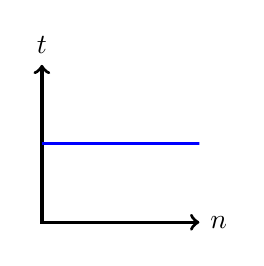
\begin{tikzpicture}
        \draw[very thick, <->] (2, 0) node[right] {\(n\)} -| (0, 2) node[above] {\(t\)};
        \clip (0,0) rectangle (2,2);
        \draw[very thick, scale=1, domain=0:2, smooth, variable=\t, blue] plot ({\t}, {1});
    \end{tikzpicture}
\end{highlight}

\subsubsection{\(O(n)\)}\label{ssub:mkon}

A \(O(n)\) time complexity is a linear growth, that can be imagined as handing out sweets to your friends.
By doubling \(n\), we double \(t\), so this is generally considered a ``good'' growth.
\begin{highlight}{Graph of \(O(n)\)}
    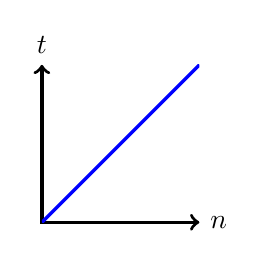
\begin{tikzpicture}
        \draw[very thick, <->] (2, 0) node[right] {\(n\)} -| (0, 2) node[above] {\(t\)};
        \clip (0,0) rectangle (2,2);
        \draw[very thick, scale=1, domain=0:2, smooth, variable=\t, blue] plot ({\t}, {\t});
    \end{tikzpicture}
\end{highlight}

\subsubsection{\(O(n^2)\)}\label{ssub:mkonsr}

This can be imagined as everyone giving everyone else a hug at a party, so for \(n\) guest, \(t\) will be \(\frac{n^2+n}{2}\).
The dominant term here is the \(n^2\), so the time complexity of the algorithm is \(O(n^2)\).

\begin{highlight}{Graph of \(O(n^2)\)}
    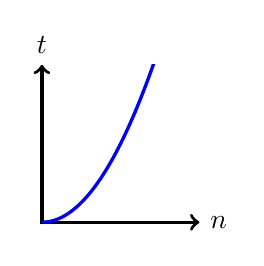
\begin{tikzpicture}
        \draw[very thick, <->] (2, 0) node[right] {\(n\)} -| (0, 2) node[above] {\(t\)};
        \clip (0,0) rectangle (2,2);
        \draw[very thick, scale=1, domain=0:2, smooth, variable=\t, blue] plot ({\t}, {\t*\t});
    \end{tikzpicture}
\end{highlight}

\subsubsection{\(O(2^{n})\)}\label{ssub:mkontwotdn}

Here we have an \emph{exponential growth}, so if \(n\) increases by \(1\), then \(t\) will double.
This is a pretty bad growth.

\begin{highlight}{Graph of \(O(2^n)\)}
    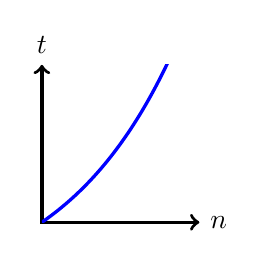
\begin{tikzpicture}
        \draw[very thick, <->] (2, 0) node[right] {\(n\)} -| (0, 2) node[above] {\(t\)};
        \clip (0,0) rectangle (2,2);
        \draw[very thick, scale=1, domain=0:2, smooth, variable=\t, blue] plot ({\t}, {2^(\t)-1});
    \end{tikzpicture}
\end{highlight}

\subsubsection{\(O(\log n)\)}\label{ssub:mkologn}

This is the inverse of the exponential function, so you have to double \(n\) to increase \(t\) by \(1\), because every step halves the remaining size.
This is a \emph{very} good time complexity.

\begin{highlight}{Graph of \(O(\log n)\)}
    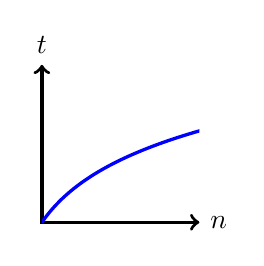
\begin{tikzpicture}
        \draw[very thick, <->] (2, 0) node[right] {\(n\)} -| (0, 2) node[above] {\(t\)};
        \clip (0,0) rectangle (2,2);
        \draw[very thick, scale=0.5, domain=0.01:6, smooth, variable=\t, blue] plot ({\t-1}, {log2(\t)});
    \end{tikzpicture}
\end{highlight}

\subsubsection{\(O(n!)\)}\label{ssub:mknfac}

A \emph{factorial} growth is \emph{very} bad because it grows \emph{very} fast.

\begin{highlight}{Graph of \(O(n!)\)}
    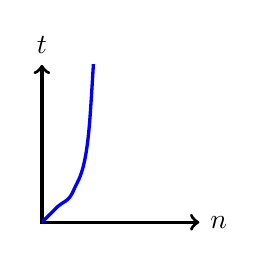
\begin{tikzpicture}
        \draw[<->, very thick] (2, 0) node[right] {\(n\)} -| (0, 2) node[above] {\(t\)};
        \clip (0,0) rectangle (2,2);
        \draw[very thick, smooth, blue] plot [smooth] coordinates{ (0, 0) (0.2, 0.2) (0.4, 0.4) (0.6, 1.2) (0.8, 4.8)};
    \end{tikzpicture}
\end{highlight}

\subsubsection{Others}\label{ssub:others}

We also have:
\begin{itemize}
    \item \(O(\sqrt{n}\) or \(O(n^{\frac{1}{2}})\) which is better than \(O(n)\), but worse than \(O(\log n)\).
    \item \(O(n \log n)\) which is sometimes called ``quasilinear'' and usually comes from having a \(O(\log n)\) operation in a \(O(n)\) loop.
\end{itemize}

\subsubsection{In Order of Goodness}\label{ssub:in_order_of_goodness}

\begin{enumerate}
    \item \(O(1)\)
    \item \(O(\log n)\)
    \item \(O(\sqrt{n})\)
    \item \(O(n)\)
    \item \(O(n \log n)\)
    \item \(O(n^2)\)
    \item \(O(n^3)\)
    \item \(O(2^{n}\)
    \item \(O(n!)\)
\end{enumerate}

\subsection{Finding The Big O Complexity}\label{sub:finding_the_big_o_complexity}

\begin{enumerate}
    \item Count the primitive operations (things like assignments, array index lookups, method calls, and returning). You should take an input \(n\), then output a function \(f(n)\). Note: remember to count operations in arrays properly.
    \item Express the number of steps as a function of \(n\) like \(T(n)=7n + 2\).
    \item Find the dominant part of the equation. We are looking at the growth rate of the function, so we can ignore all terms except the highest order one.
\end{enumerate}

\subsection{Rules for finding big O complexities}\label{sub:rules_for_finding_big_o_complexities}

\begin{enumerate}
    \item \textbf{Loops}: count the number of primitive operations as \(\mathrm{operations in loop} * \mathrm{total iterations}\)
    \item \textbf{Nested Loops}: we should analyse from the inside loop through to the outside loop, multiplying by the number of iterations each time.
    \item \textbf{Consecutive Operations}: simply add the operations
    \item \textbf{If-then-else}: have one operation for the conditional check, then assume the worst case
    \item \textbf{Constants}: remove the constant multiplier because it doesn't affect the final graph's shape
    \item Drop all lower order terms
    \item Always assume the worse case scenario
\end{enumerate}

\subsection{Big Omega}\label{sub:big_omega}

Big Omega (\(\Omega\) represents the best case scenario (ie.\ the fastest possible speed that an algorithm can perform at).
Big omega and big O can be used to calculate the enclosing bounds of the algorithm's performance.

\section{Bubble Sort}\label{sec:bubble_sort}

\begin{enumerate}
    \item Compare \(i\) with \(i+1\), swap if bigger.
    \item Repeat until the end of the array.
    \item Move the ``last index'' one position closer the start of the array so that we don't re-sort already sorted elements.
\end{enumerate}

